% AE 649 course project: Q4 plane-stress cantilever, clamp by Lagrange multipliers.
% Compile from this folder:  pdflatex presentation.tex  (twice, for the frame count)
% Every number on the slides comes from figures/*.txt (python run_all.py) or
% python -m checks.beam_theory; figures are read from ../figures/.
\documentclass[aspectratio=169,10pt]{beamer}
\usepackage[T1]{fontenc}
\usepackage{lmodern}
\usepackage{amsmath,amssymb,bm}
\usepackage{array,booktabs}
\usepackage{siunitx}
\sisetup{exponent-product=\times, group-digits=none}
\usepackage{tikz}
\usetikzlibrary{arrows.meta,patterns,calc}
\usepackage{appendixnumberbeamer}
\graphicspath{{../figures/}}
\newcolumntype{L}[1]{>{\raggedright\arraybackslash}p{#1}}

% ---------------------------------------------------------------- look
\definecolor{fblue}{HTML}{2A78D6}
\definecolor{forange}{HTML}{EB6834}
\definecolor{ink}{HTML}{0B0B0B}
\definecolor{ink2}{HTML}{52514E}
\definecolor{muted}{HTML}{898781}
\definecolor{okgreen}{HTML}{006300}

\usefonttheme[onlymath]{serif}
\setbeamertemplate{navigation symbols}{}
\setbeamercolor{normal text}{fg=ink}
\setbeamercolor{structure}{fg=fblue}
\setbeamercolor{frametitle}{fg=ink}
\setbeamercolor{title}{fg=ink}
\setbeamercolor{subtitle}{fg=ink2}
\setbeamercolor{alerted text}{fg=forange}
\setbeamercolor{block title}{fg=white,bg=fblue}
\setbeamercolor{block body}{fg=ink,bg=fblue!7}
\setbeamertemplate{blocks}[rounded][shadow=false]
\setbeamertemplate{itemize items}[circle]
\setbeamertemplate{itemize subitem}[circle]
\setbeamerfont{frametitle}{size=\large,series=\bfseries}
\setbeamertemplate{frametitle}{%
  \vspace*{0.5em}\usebeamerfont{frametitle}\insertframetitle\par
  \vspace*{-0.45em}{\color{fblue}\rule{\dimexpr\textwidth-1.1cm\relax}{0.7pt}}}
% IIT Bombay logo in the top-right corner of every slide, level with the frame title
% (an overlay, so it takes no space from the slide content). Logo: slides/iitb_logo.png, the 500 px
% PNG rendering of English Wikipedia's "Indian Institute of Technology Bombay Logo.svg" (source: iitb.ac.in).
% If the file is missing, the slides compile without the logo.
\setbeamertemplate{headline}{%
  \begin{tikzpicture}[remember picture, overlay]
    \node[anchor=north east, inner sep=0pt] at ([xshift=-0.45cm, yshift=-0.2cm]current page.north east)
      {\IfFileExists{iitb_logo.png}{\includegraphics[height=0.85cm]{iitb_logo}}{}};
  \end{tikzpicture}}
\setbeamertemplate{footline}{%
  \hspace*{1.2em}{\color{muted}\tiny Akhil S.\ Pillai \quad AE 649 \quad
  Q4 cantilever with a Lagrange-multiplier clamp\hfill\insertframenumber\,/\,\inserttotalframenumber}%
  \hspace*{1.2em}\par\vspace*{0.7em}}
\setlength{\abovedisplayskip}{3pt}
\setlength{\belowdisplayskip}{3pt}

% ---------------------------------------------------------------- notation
\newcommand{\vd}{\mathbf d}
\newcommand{\vf}{\mathbf f}
\newcommand{\vg}{\mathbf g}
\newcommand{\vR}{\mathbf R}
\newcommand{\vlam}{\bm{\lambda}}
\newcommand{\vmu}{\bm{\mu}}
\newcommand{\src}[1]{{\color{muted}\scriptsize #1}}
\newcommand{\ok}{{\color{okgreen}\checkmark}}

\title{A Q4 plane-stress cantilever with the clamp\\imposed by Lagrange multipliers}
\subtitle{Theory, implementation and analytical validation}
\author{Akhil S.\ Pillai}
\institute{Department of Aerospace Engineering, IIT Bombay\\[0.2em]AE 649 course project}
\date{November 2026}

\begin{document}

% =====================================================================
\begin{frame}[plain]
  \centering
  \IfFileExists{iitb_logo.png}{\includegraphics[height=1.6cm]{iitb_logo}\par}{}
  \vspace{-1.2em}
  \titlepage
\end{frame}

\begin{frame}{Outline}
  \begin{columns}[T]
    \begin{column}{0.48\textwidth}
      \begin{enumerate}
        \item The problem and the validation plan
        \item Theory
          \begin{itemize}
            \item plane-stress elasticity, minimum potential energy
            \item the Q4 element and Gauss quadrature
            \item assembly and consistent loads
            \item the clamp by Lagrange multipliers, scaling
            \item beam theory, shear locking, convergence
          \end{itemize}
        \item Validation V1--V6
        \item Conclusions and limitations
      \end{enumerate}
    \end{column}
    \begin{column}{0.48\textwidth}
      \begin{block}{The rule followed throughout}
        Every number the code produces is paired with an \textbf{analytical counterpart},
        computed from its formula, and every pairing is an automated test
        (109 tests). Every closed form is also derived symbolically (sympy).
      \end{block}
      \vspace{0.5em}
      \src{Code: fem/ (element, assembly, Lagrange solve), checks/ (closed forms, beam theory,
      symbolic proofs), studies/ (figures), tests/.}
    \end{column}
  \end{columns}
\end{frame}

% =====================================================================
\section{Problem}

\begin{frame}{The problem}
  \begin{center}
  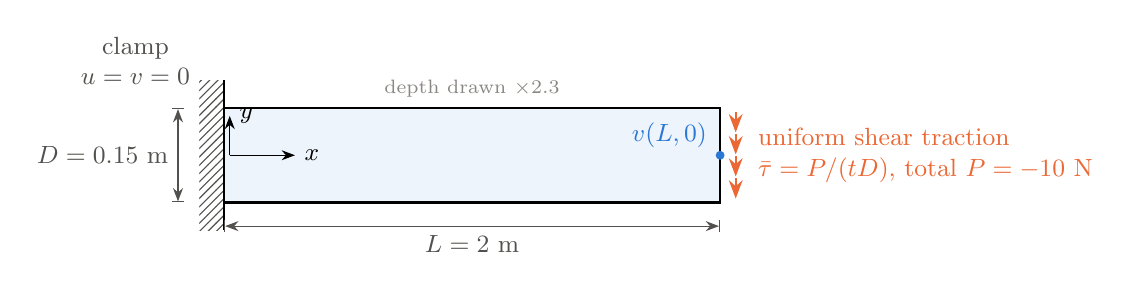
\begin{tikzpicture}[x=0.9cm,y=1cm,>=Stealth]
    \fill[pattern=north east lines, pattern color=ink2] (-0.35,-0.95) rectangle (0,0.95);
    \draw[thick] (0,-0.95) -- (0,0.95);
    \draw[thick, fill=fblue!8] (0,-0.6) rectangle (7.0,0.6);
    \foreach \yy in {-0.42,-0.14,0.14,0.42}
      \draw[->, forange, thick] (7.22,\yy+0.13) -- (7.22,\yy-0.13);
    \node[forange, right, align=left, font=\small] at (7.4,0)
      {uniform shear traction\\$\bar\tau = P/(tD)$, total $P = -10$ N};
    \draw[->] (0.08,0) -- (1.0,0) node[right, font=\small] {$x$};
    \draw[->] (0.08,0) -- (0.08,0.5) node[right, font=\small] {$y$};
    \draw[|<->|, ink2] (0,-0.9) -- (7,-0.9) node[midway, below, font=\small] {$L = 2$ m};
    \draw[|<->|, ink2] (-0.65,-0.6) -- (-0.65,0.6) node[midway, left, font=\small] {$D = 0.15$ m};
    \node[font=\small, ink2, align=center] at (-1.25,1.2) {clamp\\$u=v=0$};
    \fill[fblue] (7,0) circle (1.6pt);
    \node[fblue, font=\small, left] at (6.95,0.25) {$v(L,0)$};
    \node[muted, font=\scriptsize] at (3.5,0.85) {depth drawn $\times 2.3$};
  \end{tikzpicture}
  \end{center}
  \begin{columns}[T]
    \begin{column}{0.5\textwidth}
      \begin{itemize}
        \item Plane stress, thickness $t = 0.1$ m, $E = 200$ GPa, $\nu = 0.3$
        \item Clamp: $u = v = 0$ at \emph{every} node of $x = 0$,\\
              imposed by \textbf{Lagrange multipliers}
        \item Load: $P = -10$ N as a uniform shear traction on $x = L$
      \end{itemize}
    \end{column}
    \begin{column}{0.48\textwidth}
      \begin{itemize}
        \item Q4 elements, $2\times2$ Gauss, structured $n_x\times n_y$ meshes
        \item Nested meshes $3\times1 \to 6\times2 \to \dots \to 384\times128$\\
              (every element has $a/b = 4.44$)
        \item Outputs: tip deflection $v(L,0)$, stresses, reactions $\vR = -C^T\vlam$
      \end{itemize}
    \end{column}
  \end{columns}
\end{frame}

\begin{frame}{The validation plan: every result has an analytical counterpart}
  \small
  \begin{tabular}{@{}l L{0.25\textwidth} L{0.38\textwidth} L{0.25\textwidth}@{}}
    \toprule
    & \textbf{The code computes} & \textbf{Analytical counterpart} & \textbf{Measured agreement} \\
    \midrule
    V1 & 1D bar, both ends prescribed (Lagrange) & $u = \frac{qx(L-x)}{2EA} + \frac{Ux}{L}$; support forces from $N = EAu'$ & \num{4.8e-15}; $-\lambda = -700$, $-300$ N \\[4pt]
    V2 & Q4 stiffness, $2\times2$ Gauss & exact integration for a rectangle $2a\times2b$ & \num{2.3e-16}; 3 zero eigenvalues \\[4pt]
    V3 & uniform tension, distorted mesh & $u = \sigma_0x/E$, $v = -\nu\sigma_0y/E$ (patch test) & \num{1.1e-13} \\[4pt]
    V4 & Q4 in pure bending & Cook Eq.~3.6-11 & \num{8.6e-13} \\[4pt]
    V5 & $1\times1$ cantilever & complete hand solution (2 unknowns) & \num{1.5e-13} \\[4pt]
    V6 & $3\times1\ \dots\ 384\times128$ & statics, Clapeyron, minimum potential energy, beam theory, $O(h^2)$ & round-off; $-0.13\%$ from Timoshenko \\
    \bottomrule
  \end{tabular}
  \vspace{0.8em}

  \src{Agreement = largest relative difference between code and formula. Sources: figures/*.txt, regenerated by \texttt{python run\_all.py}.}
\end{frame}

% =====================================================================
\section{Theory}

\begin{frame}{1. Plane-stress elasticity (strong form)}
  \begin{columns}[T]
    \begin{column}{0.46\textwidth}
      \textbf{Equilibrium} (no body force)
      \[
        \frac{\partial\sigma_x}{\partial x}+\frac{\partial\tau_{xy}}{\partial y}=0,\qquad
        \frac{\partial\tau_{xy}}{\partial x}+\frac{\partial\sigma_y}{\partial y}=0
      \]
      \textbf{Strain--displacement} (small strain)
      \[
        \varepsilon_x=\frac{\partial u}{\partial x},\quad
        \varepsilon_y=\frac{\partial v}{\partial y},\quad
        \gamma_{xy}=\frac{\partial u}{\partial y}+\frac{\partial v}{\partial x}
      \]
      \textbf{Boundary conditions}\\[2pt]
      $u=v=0$ on $x=0$; traction $(0,\bar\tau)$ on $x=L$;\\
      traction-free on $y=\pm D/2$
    \end{column}
    \begin{column}{0.52\textwidth}
      \textbf{3D Hooke's law with $\sigma_z=\tau_{yz}=\tau_{zx}=0$}, solved for the stresses:
      \[
        \varepsilon_x=\frac{\sigma_x-\nu\sigma_y}{E},\qquad
        \varepsilon_y=\frac{\sigma_y-\nu\sigma_x}{E},
      \]
      \[
        \gamma_{xy}=\frac{\tau_{xy}}{G},\qquad G=\frac{E}{2(1+\nu)}
      \]
      \[
        \boxed{\begin{Bmatrix}\sigma_x\\ \sigma_y\\ \tau_{xy}\end{Bmatrix}
        =\underbrace{\frac{E}{1-\nu^2}\begin{bmatrix}1&\nu&0\\ \nu&1&0\\ 0&0&\frac{1-\nu}{2}\end{bmatrix}}_{D}
        \begin{Bmatrix}\varepsilon_x\\ \varepsilon_y\\ \gamma_{xy}\end{Bmatrix}}
      \]
      Why plane stress: the faces $z=\pm t/2$ are free, and beam theory (the reference)
      also assumes uniaxial stress, $\sigma_y=\sigma_z=0$.
    \end{column}
  \end{columns}
  \vfill
  \src{Cook Eq.~3.1-3.\ \ Code: fem/material.py.\ \ Proof: checks/derivations.py inverts the 3D compliance symbolically.}
\end{frame}

\begin{frame}{2. Principle of minimum total potential energy}
  \[
    \Pi(\mathbf u)=\frac12\int_A \bm\varepsilon^T D\,\bm\varepsilon\;t\,dA \;-\;\int_{\Gamma_t}\mathbf u^T\bar{\mathbf t}\;t\,ds
  \]
  \begin{itemize}
    \item Among displacement fields that satisfy the clamp, the exact solution makes $\Pi$ stationary
          ($\delta\Pi=0$ is the weak form of equilibrium and the traction BCs); $D$ is positive definite,
          so it is a minimum.
    \item FE approximation $\mathbf u\approx N\vd$, $\bm\varepsilon=B\vd$ in each element:
  \end{itemize}
  \[
    \Pi(\vd)=\tfrac12\,\vd^TK\vd-\vd^T\vf,\qquad
    K=\sum_e\int_{A_e}B^TDB\;t\,dA,\qquad
    \vf=\sum_e\int_{\Gamma_e}N^T\bar{\mathbf t}\;t\,ds
  \]
  \[
    \frac{\partial\Pi}{\partial\vd}=0\quad\Longrightarrow\quad K\vd=\vf\qquad\text{(supports: section 5)}
  \]
  \begin{block}{A consequence used later (V6c)}
    At the solution $\vd^TK\vd=\vf^T\vd$, so $\Pi_{\min}=-\tfrac12\,\vf^T\vd$:
    minimising $\Pi$ is the same as maximising the compliance $\vf^T\vd$.
  \end{block}
\end{frame}

\begin{frame}{3. The Q4 element: shape functions and isoparametric mapping}
  \begin{columns}[c]
    \begin{column}{0.44\textwidth}
      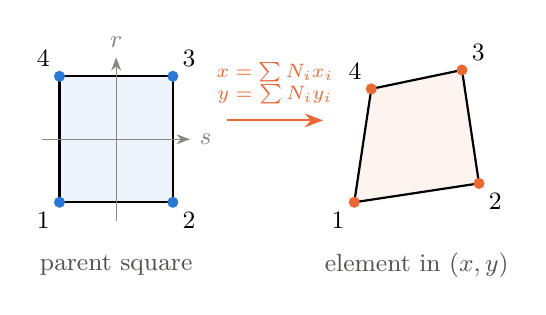
\begin{tikzpicture}[x=0.72cm,y=0.8cm,>=Stealth, font=\small]
        \draw[thick, fill=fblue!8] (-1,-1) rectangle (1,1);
        \draw[->, muted] (-1.3,0) -- (1.3,0) node[right] {$s$};
        \draw[->, muted] (0,-1.3) -- (0,1.3) node[above] {$r$};
        \foreach \xx/\yy/\n/\anc in {-1/-1/1/north east, 1/-1/2/north west, 1/1/3/south west, -1/1/4/south east}
          {\fill[fblue] (\xx,\yy) circle (2pt); \node[anchor=\anc] at (\xx,\yy) {\n};}
        \node[ink2] at (0,-2.0) {parent square};
        \draw[->, thick, forange] (1.95,0.3) -- (3.65,0.3);
        \node[forange, align=center, font=\scriptsize, anchor=south] at (2.8,0.4) {$x=\sum N_ix_i$\\$y=\sum N_iy_i$};
        \draw[thick, fill=forange!8] (4.2,-1.0) -- (6.4,-0.7) -- (6.1,1.1) -- (4.5,0.8) -- cycle;
        \foreach \xx/\yy/\n/\anc in {4.2/-1.0/1/north east, 6.4/-0.7/2/north west, 6.1/1.1/3/south west, 4.5/0.8/4/south east}
          {\fill[forange] (\xx,\yy) circle (2pt); \node[anchor=\anc] at (\xx,\yy) {\n};}
        \node[ink2] at (5.3,-2.0) {element in $(x,y)$};
      \end{tikzpicture}
    \end{column}
    \begin{column}{0.54\textwidth}
      \textbf{Bilinear shape functions} (nodes counter-clockwise)
      \[
        N_i(s,r)=\tfrac14\,(1+s\,s_i)(1+r\,r_i),\qquad s_i,r_i=\pm1
      \]
      \textbf{Isoparametric:} the same $N_i$ interpolate geometry and displacement
      \[
        x=\textstyle\sum_i N_ix_i,\quad y=\sum_i N_iy_i
      \]
      \[
        u=\textstyle\sum_i N_iu_i,\quad v=\sum_i N_iv_i
      \]
      \textbf{Properties} (tested)
      \begin{itemize}
        \item $N_i(s_j,r_j)=\delta_{ij}$: nodal values are the DOFs
        \item $\sum_i N_i=1$: rigid translations are exact
        \item ``bilinear'': a product of two 1D linear functions
      \end{itemize}
    \end{column}
  \end{columns}
  \vfill
  \src{Code: fem/q4.py (shape\_functions, shape\_derivatives).}
\end{frame}

\begin{frame}{3. The Q4 element: Jacobian, chain rule, strain--displacement matrix}
  \[
    [J]=\begin{bmatrix}x_{,s}&y_{,s}\\ x_{,r}&y_{,r}\end{bmatrix}
       =\begin{bmatrix}N_{1,s}&\cdots&N_{4,s}\\ N_{1,r}&\cdots&N_{4,r}\end{bmatrix}
        \begin{bmatrix}x_1&y_1\\ \vdots&\vdots\\ x_4&y_4\end{bmatrix},
    \qquad
    \begin{Bmatrix}N_{i,x}\\ N_{i,y}\end{Bmatrix}=[J]^{-1}\begin{Bmatrix}N_{i,s}\\ N_{i,r}\end{Bmatrix}
  \]
  \[
    \bm\varepsilon=B\,\vd_e,\qquad
    B=\begin{bmatrix}N_{1,x}&0&N_{2,x}&0&\cdots\\ 0&N_{1,y}&0&N_{2,y}&\cdots\\ N_{1,y}&N_{1,x}&N_{2,y}&N_{2,x}&\cdots\end{bmatrix}
  \]
  \[
    \vd_e=[u_1,v_1,u_2,v_2,u_3,v_3,u_4,v_4]^T,\qquad
    [J]^{-1}=\frac{1}{\det J}\begin{bmatrix}y_{,r}&-y_{,s}\\ -x_{,r}&x_{,s}\end{bmatrix}
  \]
  \begin{itemize}
    \item $dA=\det J\;ds\,dr$; the code requires $\det J>0$ (clockwise or badly distorted elements are rejected)
    \item Rectangle $2a\times2b$: $J=\operatorname{diag}(a,b)$ and $\det J=ab=$ area$/4$ \ (tested)
  \end{itemize}
  \vfill
  \src{Code: fem/q4.py (jacobian, strain\_displacement); the same lines work for one element or for all elements at once.}
\end{frame}

\begin{frame}{3. The Q4 element: stiffness and Gauss quadrature}
  \[
    k=t\int_{-1}^{1}\!\!\int_{-1}^{1}B^TDB\,\det J\;ds\,dr
    \;\approx\;t\sum_{i=1}^{2}\sum_{j=1}^{2}B^TDB\,\det J\;w_iw_j
  \]
  with the $2\times2$ Gauss points $s_i,r_j=\pm1/\sqrt3$ and weights $w_i=w_j=1$.
  \begin{columns}[T]
    \begin{column}{0.55\textwidth}
      \begin{block}{Why $2\times2$ Gauss is exact for a rectangle}
        An $n$-point rule is exact for polynomials of degree $\le 2n-1$ (here 3).
        With $x=as$, $y=br$: $N_{i,x}=\frac{s_i(1+rr_i)}{4a}$ is linear in $r$ only,
        $N_{i,y}=\frac{r_i(1+ss_i)}{4b}$ linear in $s$ only, and $\det J=ab$.
        So every entry of $B^TDB$ is at most quadratic in $s$ and in $r$: exact.\\[2pt]
        General quadrilateral: $J^{-1}$ makes the integrand rational, so Gauss is approximate.
      \end{block}
    \end{column}
    \begin{column}{0.43\textwidth}
      \textbf{Closed form by hand} (Cook \S3.6):
      \[
        k_{11}=\frac{Et}{1-\nu^2}\Big[\frac{b}{3a}+\frac{(1-\nu)a}{6b}\Big]
      \]
      \[
        k_{12}=\frac{Et}{8(1-\nu)}
      \]
      All 64 entries follow from
      $\int N_{i,x}N_{j,x}\,dA=\frac{b}{4a}s_is_j\big(1+\frac{r_ir_j}{3}\big)$ and two similar integrals.
      $k$ depends only on $a/b$, not on the element size.
    \end{column}
  \end{columns}
  \vfill
  \src{Code: fem/q4.py (gauss\_rule, element\_stiffness). Closed form: checks/closed\_form.py. Proof that $2\times2$ Gauss is exact: checks/derivations.py.}
\end{frame}

\begin{frame}{3. The Q4 element: zero-energy modes, rank and completeness}
  \begin{itemize}
    \item \textbf{Rigid-body modes.} Translations and the rotation $u=-\theta y,\ v=\theta x$ give
          $\varepsilon_x=\varepsilon_y=0$, $\gamma_{xy}=-\theta+\theta=0$, so $k\,\vd_{\text{rigid}}=\mathbf 0$:
          \textbf{3 zero eigenvalues}.
    \item \textbf{Rank.} Each Gauss point adds rank $\le 3$. With $2\times2$ the rank is $8-3=5$: no spurious modes.
          One point gives rank $\le3$, i.e.\ 2 extra zero-energy ``hourglass'' modes. Hence full integration.
    \item \textbf{Completeness.} $\sum N_i=1$, $\sum N_ix_i=x$, $\sum N_iy_i=y$ on \emph{any} quadrilateral, so every
          linear field $u=a_0+a_1x+a_2y$ is represented exactly: every constant strain is exact.
  \end{itemize}
  \begin{block}{Why the patch test (V3) must pass on distorted meshes}
    $\det J\,[N_{i,x},N_{i,y}]^T=\operatorname{adj}(J)\,[N_{i,s},N_{i,r}]^T$ is \emph{bilinear} in $(s,r)$.
    For a constant stress the nodal forces $t\int B^T\bm\sigma\det J\,ds\,dr$ are therefore integrated exactly by
    $2\times2$ Gauss. They equal the consistent loads of the boundary tractions, so the exact linear field
    satisfies the discrete equations exactly.
  \end{block}
\end{frame}

\begin{frame}{4. Assembly and consistent loads}
  \begin{columns}[T]
    \begin{column}{0.6\textwidth}
      \textbf{Assembly.} Node $n$ owns the global DOFs $2n$ ($u$) and $2n+1$ ($v$):
      \[
        K=\sum_e L_e^T\,k_e\,L_e\qquad(L_e\text{ picks the element's 8 DOFs})
      \]
      Code: 64 (row, column, value) triplets per element; COO $\to$ CSR adds the duplicates $=$ this sum.\\[5pt]
      \textbf{Consistent load of a uniform traction.} On an edge of length $h$,
      $N_{1,2}=(1\mp\xi)/2$ and $ds=\frac h2d\xi$:
      \[
        f_i=t\int N_i\,\bar\tau\,ds=\frac{t\,h\,\bar\tau}{2}\quad\text{at each end of the edge}
      \]
      With $\bar\tau=P/(tD)$ and $h=D/n_y$: $P/n_y$ at the interior end nodes and $P/(2n_y)$ at the
      two corners; the sum is $P$ (tested).
    \end{column}
    \begin{column}{0.38\textwidth}
      \centering
      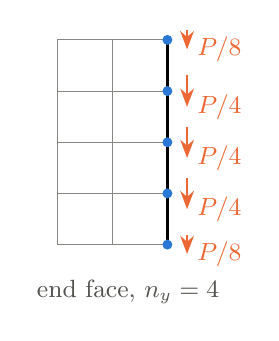
\begin{tikzpicture}[x=1cm,y=1cm,>=Stealth, font=\small]
        \foreach \j in {0,...,4} \draw[muted] (0,\j*0.65) -- (1.4,\j*0.65);
        \draw[muted] (0,0) -- (0,2.6); \draw[muted] (0.7,0) -- (0.7,2.6);
        \draw[thick] (1.4,0) -- (1.4,2.6);
        \foreach \j in {0,...,4} \fill[fblue] (1.4,\j*0.65) circle (1.8pt);
        \draw[->, forange, thick] (1.65,0.12) -- (1.65,-0.12) node[right] {$P/8$};
        \foreach \j in {1,2,3} \draw[->, forange, thick] (1.65,\j*0.65+0.2) -- (1.65,\j*0.65-0.2) node[right] {$P/4$};
        \draw[->, forange, thick] (1.65,2.72) -- (1.65,2.48) node[right] {$P/8$};
        \node[ink2] at (0.9,-0.6) {end face, $n_y=4$};
      \end{tikzpicture}

      \vspace{0.4em}
      \small\raggedright
      \textbf{Tip deflection} $v(L,0)$: the mid-height end node ($n_y$ even); for $n_y=1$, linear
      interpolation along the edge (the mean of the two end nodes).
    \end{column}
  \end{columns}
  \vfill
  \src{Code: fem/mesh.py, fem/assemble.py, fem/loads.py, fem/post.py (tip\_deflection).}
\end{frame}

\begin{frame}{5. The clamp by Lagrange multipliers}
  \textbf{Constraints}, one row per clamped DOF ($m=2(n_y+1)$ rows; each row of $C$ holds a single 1):
  \[
    C\vd=\vg\qquad(\text{clamp: }\vg=\mathbf 0;\ \text{V1 and V3 also use }\vg\ne\mathbf 0)
  \]
  \textbf{Augmented functional}
  \[
    \Pi^*(\vd,\vlam)=\tfrac12\,\vd^TK\vd-\vd^T\vf+\vlam^T(C\vd-\vg)
  \]
  \textbf{Stationarity}
  \[
    \frac{\partial\Pi^*}{\partial\vd}=\mathbf 0:\ K\vd+C^T\vlam=\vf,\qquad
    \frac{\partial\Pi^*}{\partial\vlam}=\mathbf 0:\ C\vd=\vg
    \qquad\Longrightarrow\qquad
    \boxed{\begin{bmatrix}K&C^T\\ C&0\end{bmatrix}\begin{Bmatrix}\vd\\ \vlam\end{Bmatrix}=\begin{Bmatrix}\vf\\ \vg\end{Bmatrix}}
  \]
  \begin{itemize}
    \item Size $n+m$; all DOFs stay in the system (no renumbering, no deleted rows)
    \item $K$ alone is singular (3 rigid-body modes); the augmented matrix is not
  \end{itemize}
  \vfill
  \src{Code: fem/lagrange.py (constraint\_matrix, augmented\_matrix, solve\_lagrange).}
\end{frame}

\begin{frame}{5. Properties of the saddle-point system}
  \begin{columns}[T]
    \begin{column}{0.5\textwidth}
      \textbf{Indefinite, so no Cholesky}\\[2pt]
      $\mathbf x=[\mathbf 0;\vmu]$: $\ \mathbf x^TA\mathbf x=0$ with $\mathbf x\ne\mathbf 0$.\\
      $\mathbf x=[C^T\vmu;\,-\alpha\vmu]$: $\ \mathbf x^TA\mathbf x=\vmu^TCKC^T\vmu-2\alpha\,\|C^T\vmu\|^2<0$
      for large $\alpha$.\\[3pt]
      So $A$ is not positive definite: we use sparse LU with pivoting
      (SuperLU, minimum-degree ordering on $A+A^T$).\\[6pt]
      \textbf{Nonsingular} when $C$ has full row rank and $K$ is positive definite on the null space of
      $C$ (the clamp removes all rigid-body modes). Then $A$ has exactly \textbf{$n$ positive and $m$ negative}
      eigenvalues (checked on $3\times1$, $6\times2$, $12\times4$).
    \end{column}
    \begin{column}{0.48\textwidth}
      \begin{block}{The multipliers are the reactions}
        First block row: $K\vd+C^T\vlam=\vf$. Discrete equilibrium: $K\vd=\vf+\vR$. Hence
        \[
          \boxed{\vR=K\vd-\vf=-C^T\vlam}
        \]
        Each row of $C$ picks one DOF, so the reaction at the $i$-th clamped DOF is $-\lambda_i$:
        the force the constraint applies to enforce $C\vd=\vg$.
        No post-processing is needed.
      \end{block}
    \end{column}
  \end{columns}
\end{frame}

\begin{frame}{5. Lagrange multipliers = elimination + reactions}
  Order the DOFs as free ($f$) and constrained ($c$), so $C=[\,0\ \ I\,]$:
  \[
    \begin{bmatrix}K_{ff}&K_{fc}&0\\ K_{cf}&K_{cc}&I\\ 0&I&0\end{bmatrix}
    \begin{Bmatrix}\vd_f\\ \vd_c\\ \vlam\end{Bmatrix}
    =\begin{Bmatrix}\vf_f\\ \vf_c\\ \vg\end{Bmatrix}
  \]
  \begin{itemize}
    \item Third row: $\vd_c=\vg$
    \item First row: $\boxed{K_{ff}\,\vd_f=\vf_f-K_{fc}\,\vg}$ --- exactly the eliminated system
    \item Second row: $\vlam=\vf_c-K_{cf}\vd_f-K_{cc}\vg=-\vR_c$ --- the reactions
  \end{itemize}
  \begin{block}{So}
    Lagrange multipliers give the elimination displacements \emph{exactly}, plus the reactions, without
    removing any equation. Proved symbolically for a generic $K$ (checks/derivations.py) and checked
    numerically against elimination (written only inside the tests).
  \end{block}
\end{frame}

\begin{frame}{5. Scaling the constraint rows and columns}
  $K\sim10^{10}$ N/m but $C$ holds ones. Multiply the constraint rows \emph{and} columns by $s=\max\operatorname{diag}K$:
  \[
    \begin{bmatrix}K&sC^T\\ sC&0\end{bmatrix}\begin{Bmatrix}\vd\\ \vlam_s\end{Bmatrix}=\begin{Bmatrix}\vf\\ s\vg\end{Bmatrix},
    \qquad A_s=SAS,\ \ S=\operatorname{diag}(I,sI)
  \]
  \begin{columns}[T]
    \begin{column}{0.5\textwidth}
      \begin{itemize}
        \item Solution $S^{-1}[\vd;\vlam]$: \textbf{$\vd$ unchanged}, $\vlam_s=\vlam/s$, and
              $\vR=-(sC)^T\vlam_s=-C^T\vlam$
        \item A congruence, so the inertia is unchanged (Sylvester's law)
        \item Why $\sim10^{22}$ unscaled: $A^{-1}$ contains the block $K_{cf}K_{ff}^{-1}K_{fc}-K_{cc}$, as large
              as $K$, so $\|A\|\,\|A^{-1}\|\sim\|K\|^2$. Scaled, that block is divided by $s^2$, and
              $\operatorname{cond}(A_s)\approx\operatorname{cond}(K_{ff})$
      \end{itemize}
    \end{column}
    \begin{column}{0.48\textwidth}
      \footnotesize
      \begin{tabular}{@{}lrrr@{}}
        \toprule
        $\operatorname{cond}_2$ & unscaled & scaled & $K_{ff}$ \\
        \midrule
        $3\times1$  & \num{9.381e21} & \num{2.492e4} & \num{2.412e4} \\
        $6\times2$  & \num{2.381e22} & \num{2.746e5} & \num{2.728e5} \\
        $12\times4$ & \num{3.594e22} & \num{1.921e6} & \num{1.919e6} \\
        $24\times8$ & \num{4.170e22} & \num{9.140e6} & \num{9.139e6} \\
        \bottomrule
      \end{tabular}\\[3pt]
      \scriptsize float64 SVD, confirmed by a 50-digit SVD on the two smallest meshes.
    \end{column}
  \end{columns}
  \vfill
  \src{figures/exact\_field.txt. Digit loss: Cook \S9.3, Eq.~9.3-4: up to $\log_{10}\operatorname{cond}$ digits.}
\end{frame}

\begin{frame}{5. Scaling: the measured effect}
  \begin{columns}[c]
    \begin{column}{0.5\textwidth}
      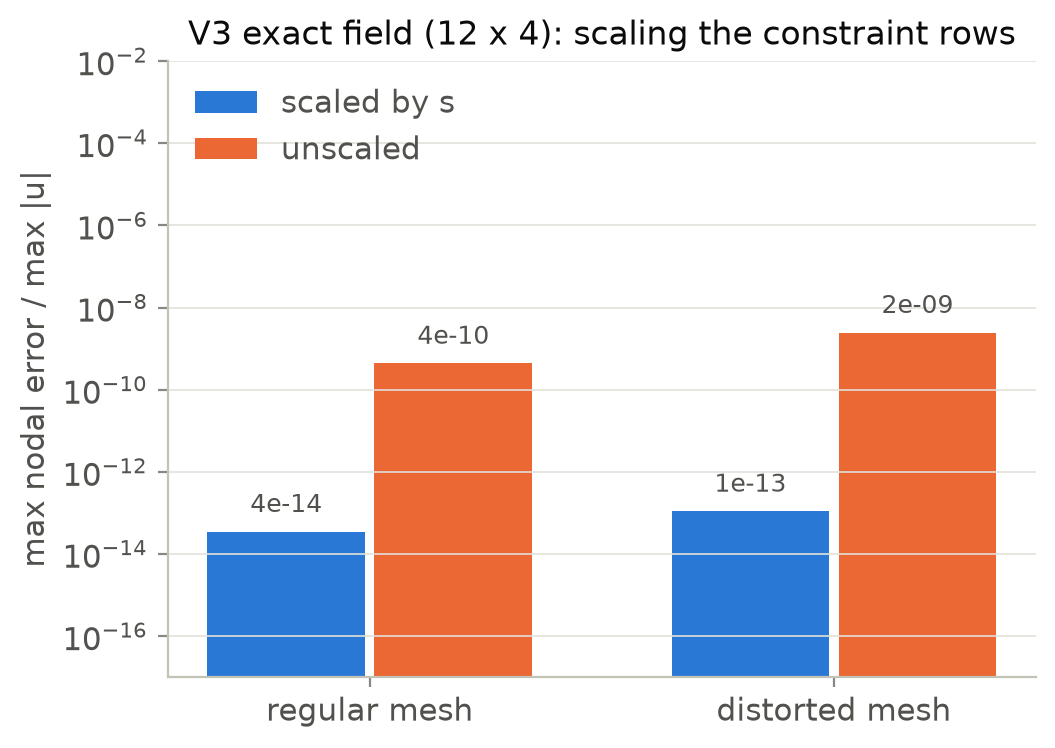
\includegraphics[width=\linewidth]{exact_field_scaling.png}
    \end{column}
    \begin{column}{0.48\textwidth}
      \begin{itemize}
        \item Exact linear field (V3, $12\times4$), relative nodal error:
              \textbf{\num{4.4e-10} unscaled vs \num{3.5e-14} scaled} (regular mesh),
              \num{2.5e-9} vs \num{1.1e-13} (distorted): about \textbf{four digits lost} without scaling
        \item Cook Eq.~9.3-4: up to $\log_{10}\operatorname{cond}$ digits may be lost:
              22 unscaled (more than float64 has), 4--7 scaled
        \item Beyond $\operatorname{cond}\approx1/\epsilon$ even eigenvalues are unreliable: on $12\times4$,
              \texttt{eigvalsh} of the unscaled matrix finds 134 positive / 6 negative instead of 130 / 10;
              the scaled matrix gives 130 / 10
      \end{itemize}
    \end{column}
  \end{columns}
  \vfill
  \src{figures/exact\_field.txt, figures/exact\_field\_scaling.png.}
\end{frame}

\begin{frame}{6. Beam-theory reference}
  \begin{columns}[T]
    \begin{column}{0.6\textwidth}
      Moment (sagging positive): $M(x)=P(L-x)$.\\[3pt]
      \textbf{Euler--Bernoulli:} $EIv''=M$, $v(0)=v'(0)=0$:
      \[
        v=\frac{P}{EI}\Big(\frac{Lx^2}{2}-\frac{x^3}{6}\Big)\ \Rightarrow\ v(L)=\frac{PL^3}{3EI},
        \qquad I=\frac{tD^3}{12}
      \]
      \textbf{Stresses:} $\sigma_{xx}=-\dfrac{My}{I}=-\dfrac{P(L-x)\,y}{I}$; equilibrium with $\tau_{xy}(\pm D/2)=0$ gives
      \[
        \tau_{xy}=\frac{P}{2I}\Big(\frac{D^2}{4}-y^2\Big),\qquad\int\tau_{xy}\,t\,dy=P
      \]
      \textbf{Timoshenko:} shear strain $V/(\kappa GA)$, $\kappa=5/6$ for a rectangle:
      \[
        v(L)=\frac{PL^3}{3EI}+\frac{PL}{\kappa GA}
      \]
    \end{column}
    \begin{column}{0.38\textwidth}
      \begin{block}{Values}
        $I=\num{2.8125e-5}$ m$^4$\\
        Euler--Bernoulli: \textbf{$-4.74074$ \textmu m}\\
        shear term: $-0.02080$ \textmu m (0.44\%)\\
        Timoshenko: \textbf{$-4.76154$ \textmu m}\\
        $\sigma_{xx}(L/2,\pm D/2)=\pm26.6667$ kPa
      \end{block}
      \small
      Stresses are compared at mid-span, 6.7 depths from either end, where Saint-Venant end effects have
      decayed. Beam theory needs only the resultant $P$.
    \end{column}
  \end{columns}
  \vfill
  \src{Values: \texttt{python -m checks.beam\_theory}. All derived symbolically in checks/derivations.py. $\kappa=5/6$: Cook p.~535.}
\end{frame}

\begin{frame}{7. Why Q4 is stiff in bending: parasitic shear (Cook \S3.6)}
  \begin{columns}[T]
    \begin{column}{0.5\textwidth}
      \textbf{Block in pure bending} (Cook Eq.~3.6-9):
      \[
        \varepsilon_x=-\frac{\theta y}{2a},\quad\varepsilon_y=\nu\frac{\theta y}{2a},\quad\gamma_{xy}=0
      \]
      \textbf{Q4 bent the same way} (sides stay straight, Eq.~3.6-10):
      \[
        \varepsilon_x=-\frac{\theta y}{2a},\quad\varepsilon_y=0,\quad\gamma_{xy}=\color{forange}-\frac{\theta x}{2a}
      \]
      Strain energies:
      \[
        U_b=\frac{Et\,\theta^2b^3}{6a},\qquad U_{el}=\frac{t\,\theta^2b}{6a}\Big[\frac{Eb^2}{1-\nu^2}+Ga^2\Big]
      \]
    \end{column}
    \begin{column}{0.48\textwidth}
      At equal moment $U=M\theta/2=k\theta^2/2$, so $\theta_{el}/\theta_b=U_b/U_{el}$:
      \[
        \boxed{\frac{\theta_{FE}}{\theta_{exact}}=\frac{1-\nu^2}{1+\frac{1-\nu}{2}\big(\frac ab\big)^2}}
      \]
      \small Cook Eq.~3.6-11, p.~99; $a,b$ = element half-length and half-depth.
      \begin{itemize}
        \item $1-\nu^2$: from $\varepsilon_y=0$
        \item $(a/b)^2$: only from the parasitic shear: \textbf{shear locking}
        \item $a/b=1$: 0.674; our elements ($a/b=4.44$): 0.115; one element for the whole beam ($a/b=13.3$): 0.0144
      \end{itemize}
    \end{column}
  \end{columns}
  \vfill
  \src{Energies and Eq.~3.6-11 derived symbolically in checks/derivations.py; values from figures/bending\_error.txt.}
\end{frame}

\begin{frame}{8. Convergence theory}
  \begin{columns}[T]
    \begin{column}{0.5\textwidth}
      \textbf{Monotone compliance} (minimum potential energy).
      Each mesh subdivides the previous one, so the displacement spaces are nested, $V_h\subset V_{h/2}$
      (the coarse clamp is zero along the whole edge). A larger space cannot give a larger minimum:
      $\Pi_{h/2}\le\Pi_h$, and with $\Pi_{\min}=-\frac12\vf^T\vd$:
      \[
        \vf^T\vd_h\ \le\ \vf^T\vd_{h/2}\ \le\ \text{exact compliance}
      \]
      The FE model is too stiff and can only soften under refinement.\\[4pt]
      \textbf{Rate.} Bilinear elements, smooth solution: energy error $O(h)$; displacements and outputs
      such as $v(L,0)$: $O(h^2)$.
    \end{column}
    \begin{column}{0.48\textwidth}
      \textbf{Observed order} from three nested meshes, $\phi=\phi_\infty+c\,h^q$:
      \[
        \frac{\phi_1-\phi_2}{\phi_2-\phi_3}=2^q\ \Rightarrow\ q=\log_2\frac{\phi_1-\phi_2}{\phi_2-\phi_3}
      \]
      \textbf{Richardson extrapolation} (Cook Eq.~9.7-1):
      \[
        \phi_\infty=\frac{2^q\,\phi_{h/2}-\phi_h}{2^q-1}
      \]
      Valid for regular nested refinement with the quantity at a fixed node (both hold here).\\[4pt]
      Caveat: the clamped corners are singular points of the 2D solution and could lower the
      asymptotic rate on much finer meshes.
    \end{column}
  \end{columns}
  \vfill
  \src{Code: fem/post.py (observed\_order, richardson); formulas proved in checks/derivations.py.}
\end{frame}

% =====================================================================
\section{Validation}

\begin{frame}{V1: 1D bar, both ends prescribed --- the Lagrange machinery alone}
  \begin{columns}[c]
    \begin{column}{0.55\textwidth}
      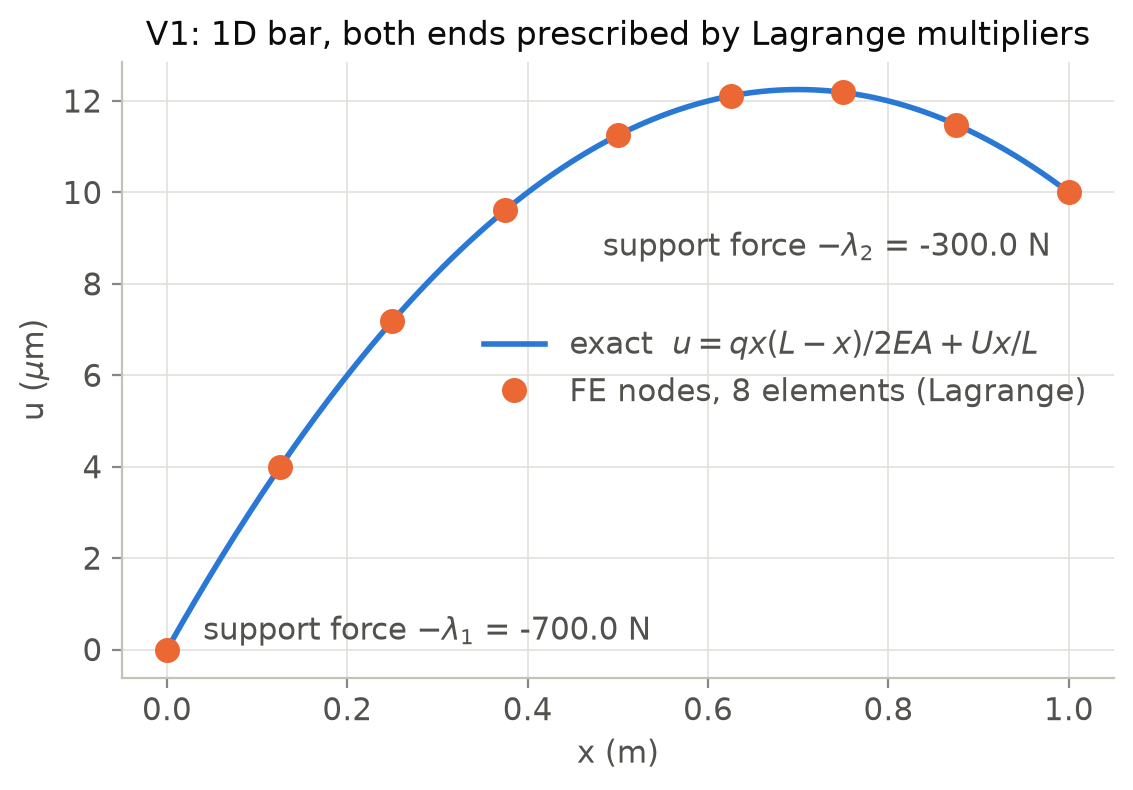
\includegraphics[width=\linewidth]{bar1d.png}
    \end{column}
    \begin{column}{0.43\textwidth}
      $EAu''+q=0$, $u(0)=0$, $u(L)=U$:
      \[
        u=\frac{qx(L-x)}{2EA}+\frac{Ux}{L},\qquad N=EAu'
      \]
      Support forces: $-N(0)$ and $+N(L)$.\\[3pt]
      Linear elements with constant $EA$ and consistent loads are \textbf{nodally exact} (Cook p.~47): the Green's
      function of a nodal load is piecewise linear, so Galerkin orthogonality makes the nodal error zero.\\[4pt]
      Max nodal error on 2, 3, 8, 32 elements: $\le\num{4.8e-15}$ \ok\\[2pt]
      $-\lambda_1=-700$ N, $-\lambda_2=-300$ N $=$ the exact support forces \ok
    \end{column}
  \end{columns}
  \vfill
  \src{$L=1$ m, $EA=2\times10^7$ N, $q=1000$ N/m, $U=10^{-5}$ m. Same solver as the 2D problem. figures/bar1d.txt.}
\end{frame}

\begin{frame}{V2: the Q4 element stiffness}
  \begin{columns}[c]
    \begin{column}{0.52\textwidth}
      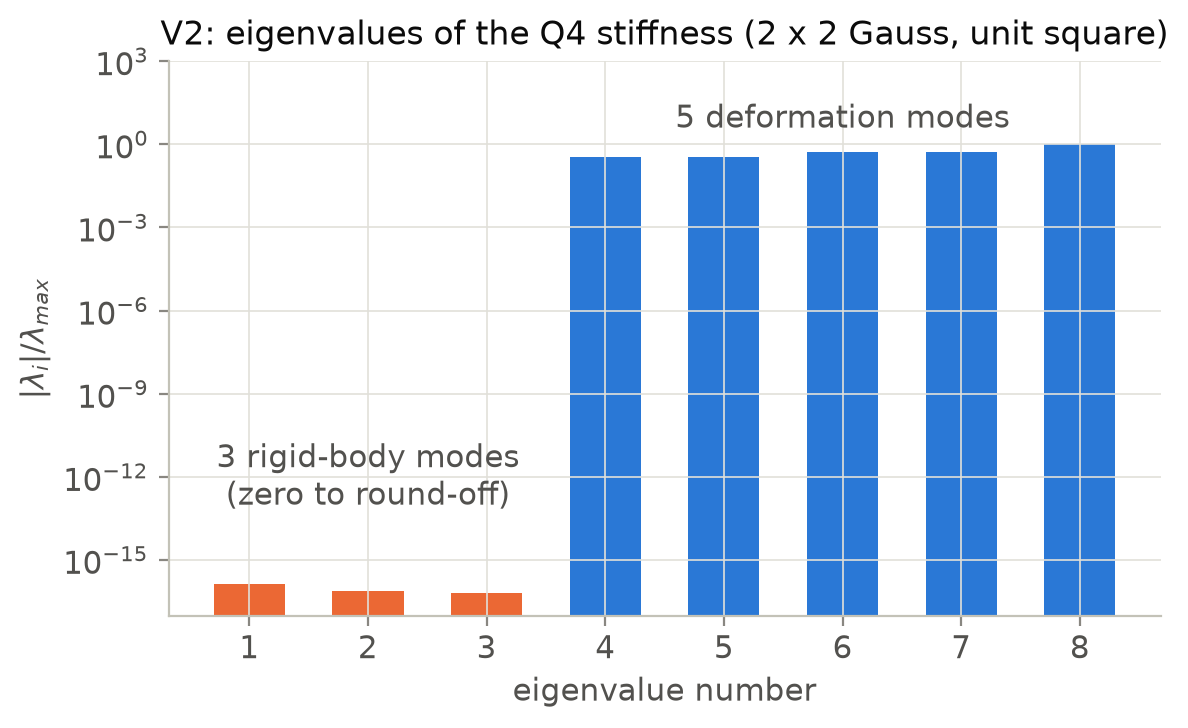
\includegraphics[width=\linewidth]{element_checks.png}
    \end{column}
    \begin{column}{0.46\textwidth}
      \begin{tabular}{@{}ll@{}}
        \toprule
        unit square & N/m \\
        \midrule
        $k_{11}$, code    & \num{9.8901098901e9} \\
        $k_{11}$, formula & \num{9.8901098901e9} \\
        $k_{12}$, code    & \num{3.5714285714e9} \\
        $k_{12}$, formula & \num{3.5714285714e9} \\
        \bottomrule
      \end{tabular}
      \begin{itemize}
        \item All 64 entries equal exact integration to $\le\num{2.3e-16}$ (4 rectangles) \ok
        \item $2\times2$ vs $3\times3$ Gauss: $\le\num{7.7e-16}$ for rectangles, \num{8.3e-3} for a general
              quadrilateral (integrand no longer polynomial)
        \item Exactly \textbf{3 zero eigenvalues} ($|\lambda|/\lambda_{\max}\le\num{1.3e-16}$) and
              5 deformation modes \ok
      \end{itemize}
    \end{column}
  \end{columns}
  \vfill
  \src{$t=0.1$ m. figures/element\_checks.txt.}
\end{frame}

\begin{frame}{V3: uniform tension --- an exact linear field (patch test)}
  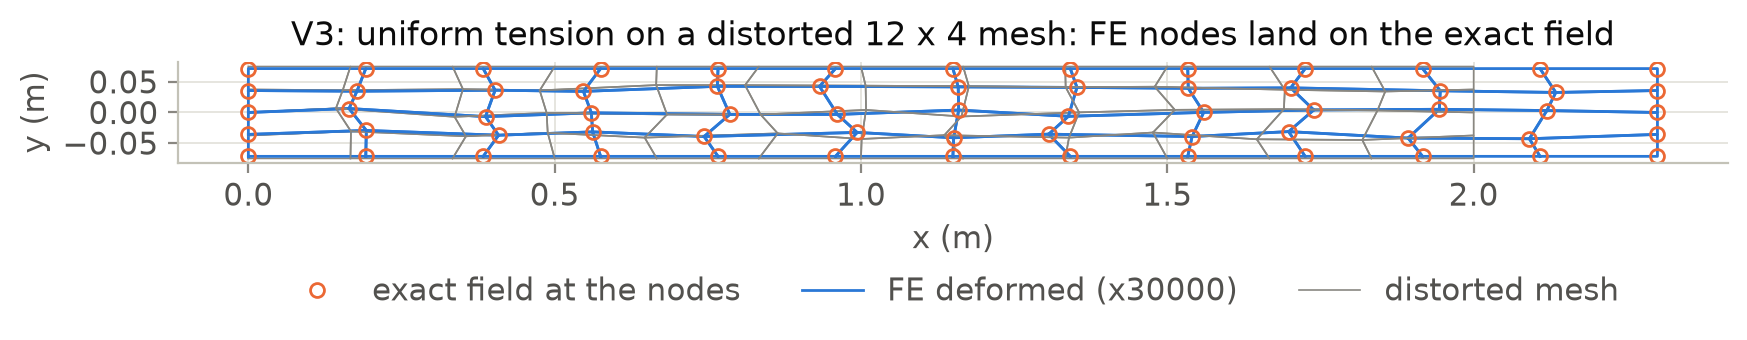
\includegraphics[width=\linewidth]{exact_field.png}
  \begin{columns}[T]
    \begin{column}{0.5\textwidth}
      $u=\sigma_0x/E$, $v=-\nu\sigma_0y/E$ gives $\bm\sigma=[\sigma_0,0,0]$ everywhere: equilibrium, free top and
      bottom, $u=0$ on $x=0$, $v=0$ at $(0,0)$. All supports by Lagrange multipliers. Q4 contains every linear
      field, so the FE answer must be \textbf{exact} on any mesh.
    \end{column}
    \begin{column}{0.48\textwidth}
      \begin{tabular}{@{}lrr@{}}
        \toprule
        $12\times4$ & nodal error & stress error \\
        \midrule
        regular   & \num{3.5e-14} & \num{2.6e-14} \\
        distorted & \num{1.1e-13} & \num{4.9e-14} \\
        \bottomrule
      \end{tabular}\\[3pt]
      Reactions $=$ minus the consistent loads of $\sigma_0$ on the left edge \ok\\
      Also with $\vg\ne\mathbf 0$ (exact field plus a rigid motion) \ok
    \end{column}
  \end{columns}
  \vfill
  \src{figures/exact\_field.txt; tests/test\_exact\_field.py.}
\end{frame}

\begin{frame}{V4: Q4 in pure bending against Cook Eq.~3.6-11}
  \begin{columns}[c]
    \begin{column}{0.55\textwidth}
      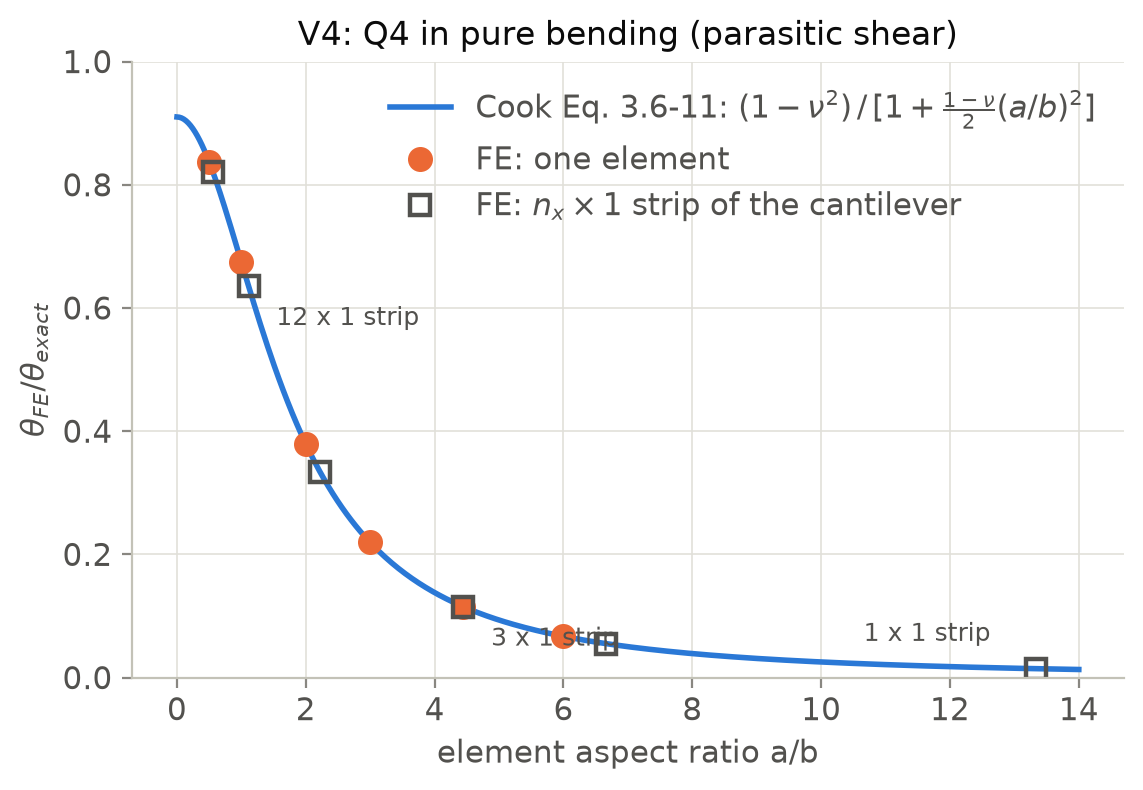
\includegraphics[width=\linewidth]{bending_error.png}
    \end{column}
    \begin{column}{0.43\textwidth}
      One clamped element under an end couple, and $n_x\times1$ strips of the cantilever. Every element of a strip
      carries the same moment, so a strip behaves \emph{exactly} like one element with $a=L/(2n_x)$.\\[5pt]
      \begin{tabular}{@{}lrr@{}}
        \toprule
        case & $a/b$ & $\theta_{FE}/\theta_{exact}$ \\
        \midrule
        one element & 1 & 0.6740740741 \\
        $3\times1$ strip & 4.44 & 0.1149921997 \\
        $1\times1$ strip & 13.3 & 0.0143936731 \\
        \bottomrule
      \end{tabular}\\[4pt]
      FE $=$ formula to $\le\num{8.6e-13}$ in all 12 cases \ok\\[3pt]
      This is why the coarse meshes are so stiff.
    \end{column}
  \end{columns}
  \vfill
  \src{figures/bending\_error.txt.}
\end{frame}

\begin{frame}{V5: one-element cantilever, solved completely by hand}
  \begin{columns}[c]
    \begin{column}{0.47\textwidth}
      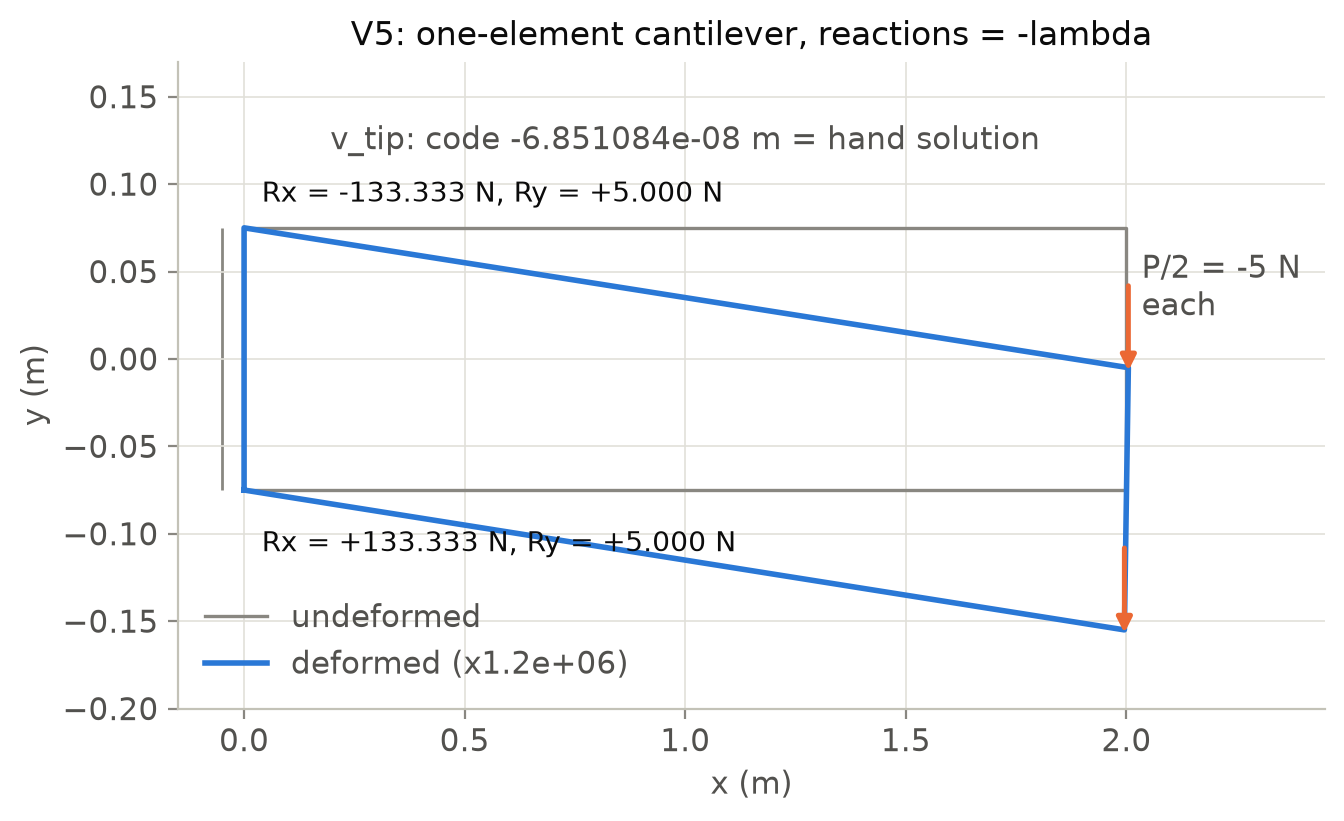
\includegraphics[width=\linewidth]{one_element.png}
    \end{column}
    \begin{column}{0.51\textwidth}
      Symmetry ($u$ odd, $v$ even in $y$) leaves 2 unknowns. Minimising $\Pi(q,w)$:
      \[
        v_{tip}=\frac{4PL(1+\nu)\left[2L^2(1-\nu)+D^2\right]}{EtD\left[L^2(1-\nu)+2D^2\right]}
      \]
      $\sum F_x=0$, $\sum M=0$: $R_x=-PL/D$ (bottom), $+PL/D$ (top);
      $\sum F_y=0$ \emph{plus symmetry}: $R_y=-P/2$ each.\\[3pt]
      \small
      \begin{tabular}{@{}lr@{}}
        \toprule
        $v_{tip}$ (code $=$ hand) & \num{-6.8510837727e-8} m \\
        $u$ top / bottom & $\pm\num{3.8383128295e-9}$ m \\
        $R_x$ bottom / top & $+133.333$ / $-133.333$ N \\
        $R_y$ each & $+5.000$ N \\
        \bottomrule
      \end{tabular}\\[2pt]
      Code $=$ hand solution to $\le\num{1.5e-13}$, and $\vlam=-\vR$ \ok\\
      $v_{tip}$ is only 0.01445 of Euler--Bernoulli: locking.
    \end{column}
  \end{columns}
  \vfill
  \src{figures/one\_element.txt. checks/derivations.py re-derives it over all four free DOFs, without assuming symmetry.}
\end{frame}

\begin{frame}{V6 (a, b): statics and Clapeyron on every mesh}
  \small
  \begin{tabular}{@{}lrrrr@{}}
    \toprule
    mesh & $\sum R_x$ (N) & $\sum R_y$ (N) & moment of $\vR$ (N\,m) & Clapeyron, relative \\
    \midrule
    $3\times1$     & \num{1.1e-12}  & 9.999999999979  & 19.999999999970 & \num{1.6e-13} \\
    $12\times4$    & \num{-2.3e-11} & 9.999999999496  & 19.999999999379 & \num{3.1e-11} \\
    $48\times16$   & \num{9.2e-12}  & 9.999999998828  & 19.999999999391 & \num{2.2e-11} \\
    $192\times64$  & \num{2.2e-10}  & 10.000000007987 & 20.000000008089 & \num{-7.3e-10} \\
    $384\times128$ & \num{1.1e-9}   & 9.999999980917  & 19.999999961142 & \num{1.4e-9} \\
    \midrule
    \textbf{theory} & 0 & $-P=10$ & $-PL=20$ & 0 \\
    \bottomrule
  \end{tabular}\\[2pt]
  \scriptsize Moment about $(0,0)$. Clapeyron: $(\vd^TK\vd-\vf^T\vd)/\vf^T\vd$.
  \normalsize
  \vspace{0.6em}
  \begin{columns}[T]
    \begin{column}{0.49\textwidth}
      \begin{block}{Why statics is exact}
        Each $k_e$ annihilates rigid-body motions, so the nodal forces $K\vd$ are self-equilibrated, and the
        reactions $\vR=-C^T\vlam$ balance the load exactly (to round-off).
      \end{block}
    \end{column}
    \begin{column}{0.49\textwidth}
      \begin{block}{Why Clapeyron holds}
        $\vd^T(K\vd+C^T\vlam)=\vd^T\vf$ and $C\vd=\mathbf 0$, so $\vd^TK\vd=\vf^T\vd$:
        the reactions do no work.
      \end{block}
    \end{column}
  \end{columns}
  \vfill
  \src{All 8 meshes in figures/reactions.txt; the round-off grows with the condition number, as expected.}
\end{frame}

\begin{frame}{V6 (c, d): tip deflection under nested refinement}
  \begin{columns}[c]
    \begin{column}{0.55\textwidth}
      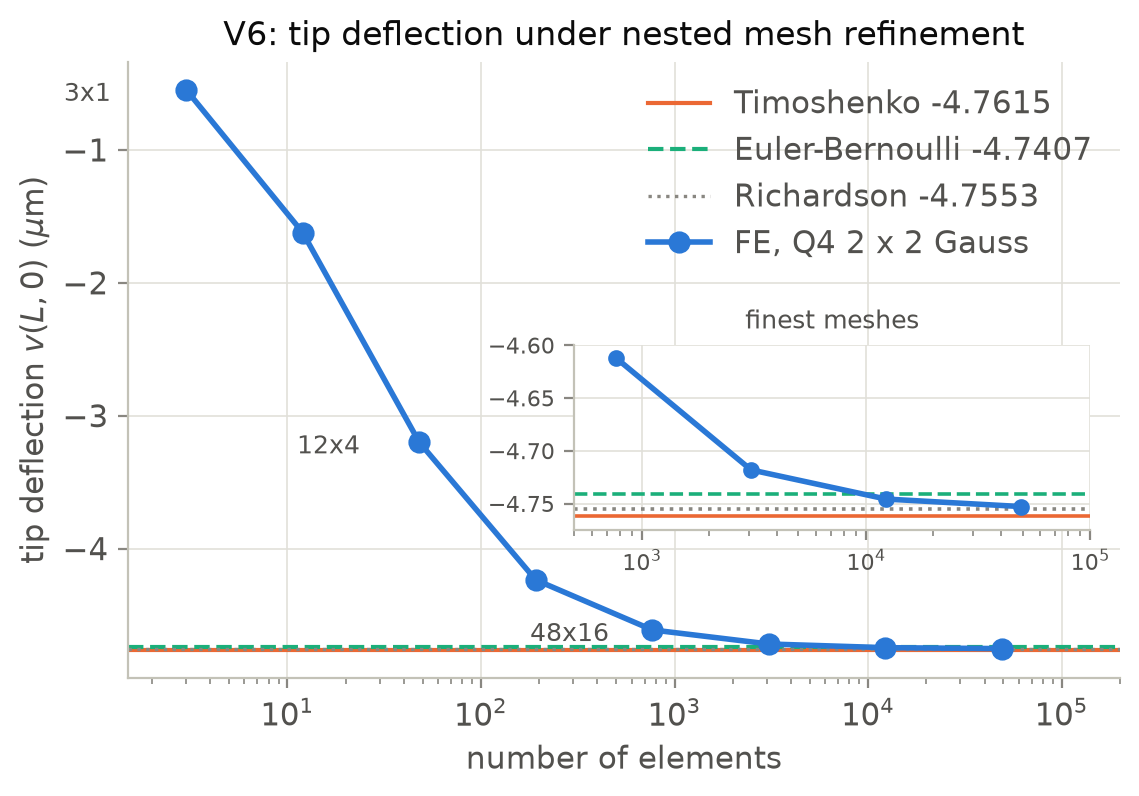
\includegraphics[width=\linewidth]{tip_deflection.png}
    \end{column}
    \begin{column}{0.43\textwidth}
      \small
      \begin{tabular}{@{}lrrr@{}}
        \toprule
        mesh & $v_{tip}$ (\textmu m) & /\,E--B & /\,Tim. \\
        \midrule
        $3\times1$     & $-0.54734$ & 0.1155 & 0.1149 \\
        $6\times2$     & $-1.62173$ & 0.3421 & 0.3406 \\
        $12\times4$    & $-3.19979$ & 0.6750 & 0.6720 \\
        $24\times8$    & $-4.23595$ & 0.8935 & 0.8896 \\
        $48\times16$   & $-4.61223$ & 0.9729 & 0.9686 \\
        $96\times32$   & $-4.71813$ & 0.9952 & 0.9909 \\
        $192\times64$  & $-4.74577$ & 1.0011 & 0.9967 \\
        $384\times128$ & $-4.75287$ & 1.0026 & 0.9982 \\
        \bottomrule
      \end{tabular}\\[4pt]
      Compliance $\vf^T\vd$ increases on every refinement \ok\\
      Equal to an independent implementation to all 5 printed digits \ok
    \end{column}
  \end{columns}
  \vfill
  \src{figures/tip\_deflection.txt.}
\end{frame}

\begin{frame}{V6 (e): observed convergence rate and Richardson extrapolation}
  \begin{columns}[c]
    \begin{column}{0.5\textwidth}
      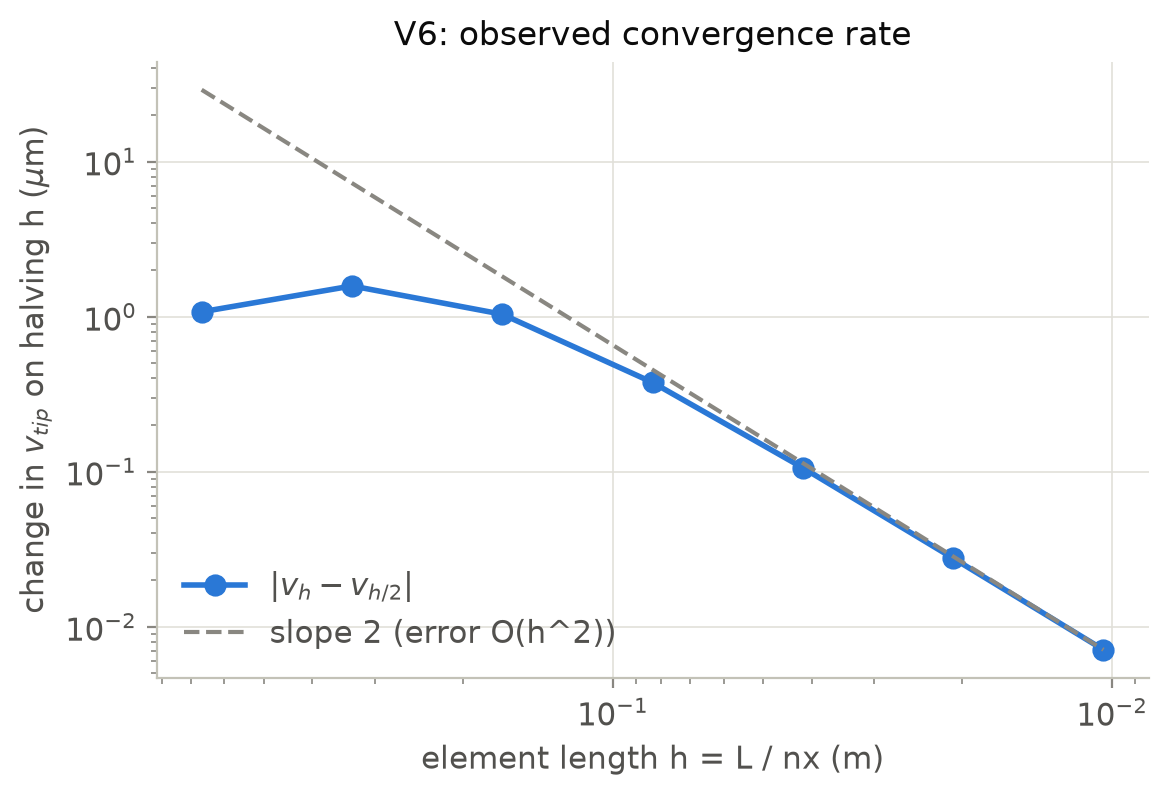
\includegraphics[width=\linewidth]{convergence_rate.png}
    \end{column}
    \begin{column}{0.48\textwidth}
      \small
      \begin{tabular}{@{}lrr@{}}
        \toprule
        finest mesh & order $q$ & Richardson (\textmu m) \\
        \midrule
        $48\times16$   & 1.461 & $-4.82679$ \\
        $96\times32$   & 1.829 & $-4.75961$ \\
        $192\times64$  & 1.938 & $-4.75553$ \\
        $384\times128$ & 1.961 & $-4.75532$ \\
        \bottomrule
      \end{tabular}\\[4pt]
      The order rises towards the theoretical 2 \ok\ (coarse meshes: locking dominates).
      \begin{block}{Converged tip deflection}
        $-4.75532$ \textmu m $=$ \textbf{0.99869 $\times$ Timoshenko} ($-0.13\%$)\\
        $=$ 1.00308 $\times$ Euler--Bernoulli ($+0.31\%$)\\
        The last two estimates differ by 0.004\%.
      \end{block}
    \end{column}
  \end{columns}
  \vfill
  \src{Each row uses three nested meshes ending at the one named (e.g.\ $48\times16$: $12\times4$, $24\times8$, $48\times16$). figures/tip\_deflection.txt.}
\end{frame}

\begin{frame}{V6 (d): bending stress at mid-span}
  \begin{columns}[c]
    \begin{column}{0.55\textwidth}
      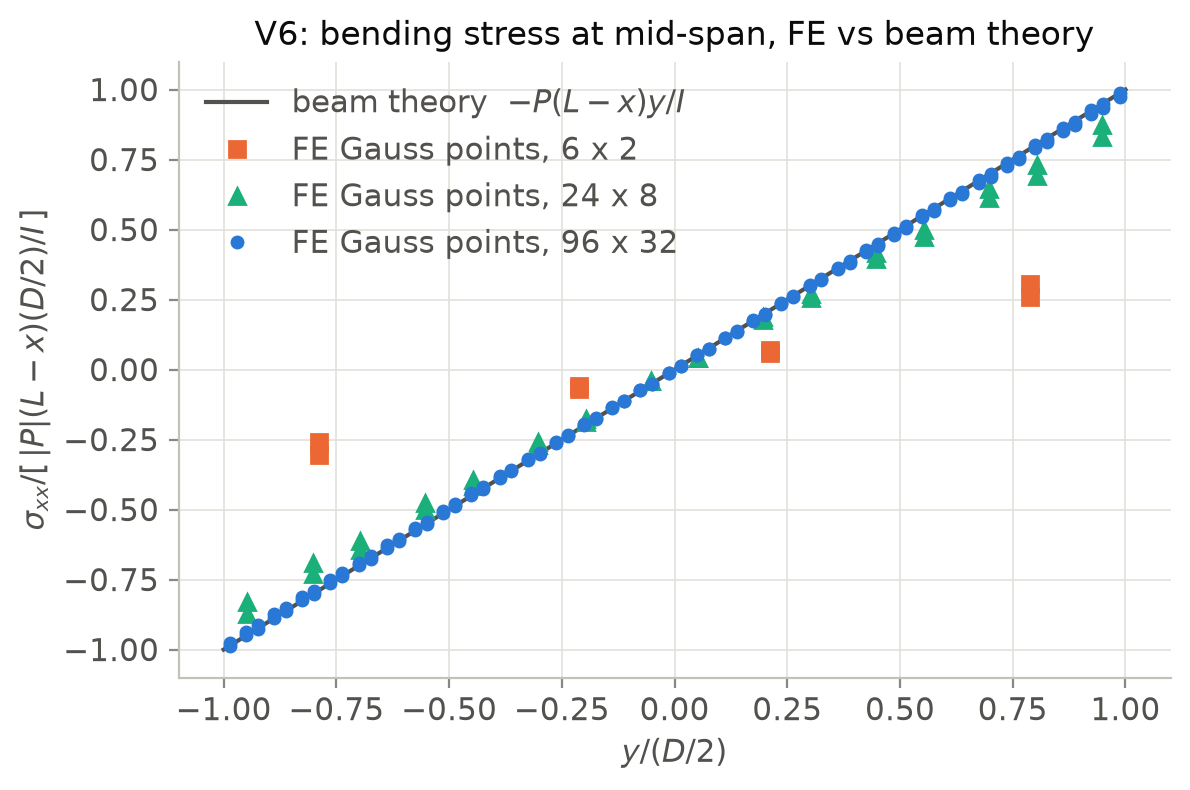
\includegraphics[width=\linewidth]{midspan_stress.png}
    \end{column}
    \begin{column}{0.43\textwidth}
      Gauss points of the element column at $x=L/2$, against $\sigma_{xx}=-P(L-x)y/I$ at the same points.
      Error: the largest $|\sigma_{FE}-\sigma_{beam}|$ over those points, divided by the beam surface stress at
      the same $x$.\\[5pt]
      \begin{tabular}{@{}lr@{}}
        \toprule
        mesh & error \\
        \midrule
        $3\times1$ / $6\times2$ & 0.5162 / 0.5308 \\
        $24\times8$ & 0.1163 \\
        $96\times32$ & 0.0150 \\
        $384\times128$ & 0.0025 \\
        \bottomrule
      \end{tabular}\\[4pt]
      Falls on every refinement from $6\times2$ on \ok\ (the two coarsest meshes are dominated by locking).
    \end{column}
  \end{columns}
  \vfill
  \src{figures/midspan\_stress.txt (all 8 meshes; equal to the independent table where it exists).}
\end{frame}

\begin{frame}{V6: reactions $\vR=-C^T\vlam$ along the clamp}
  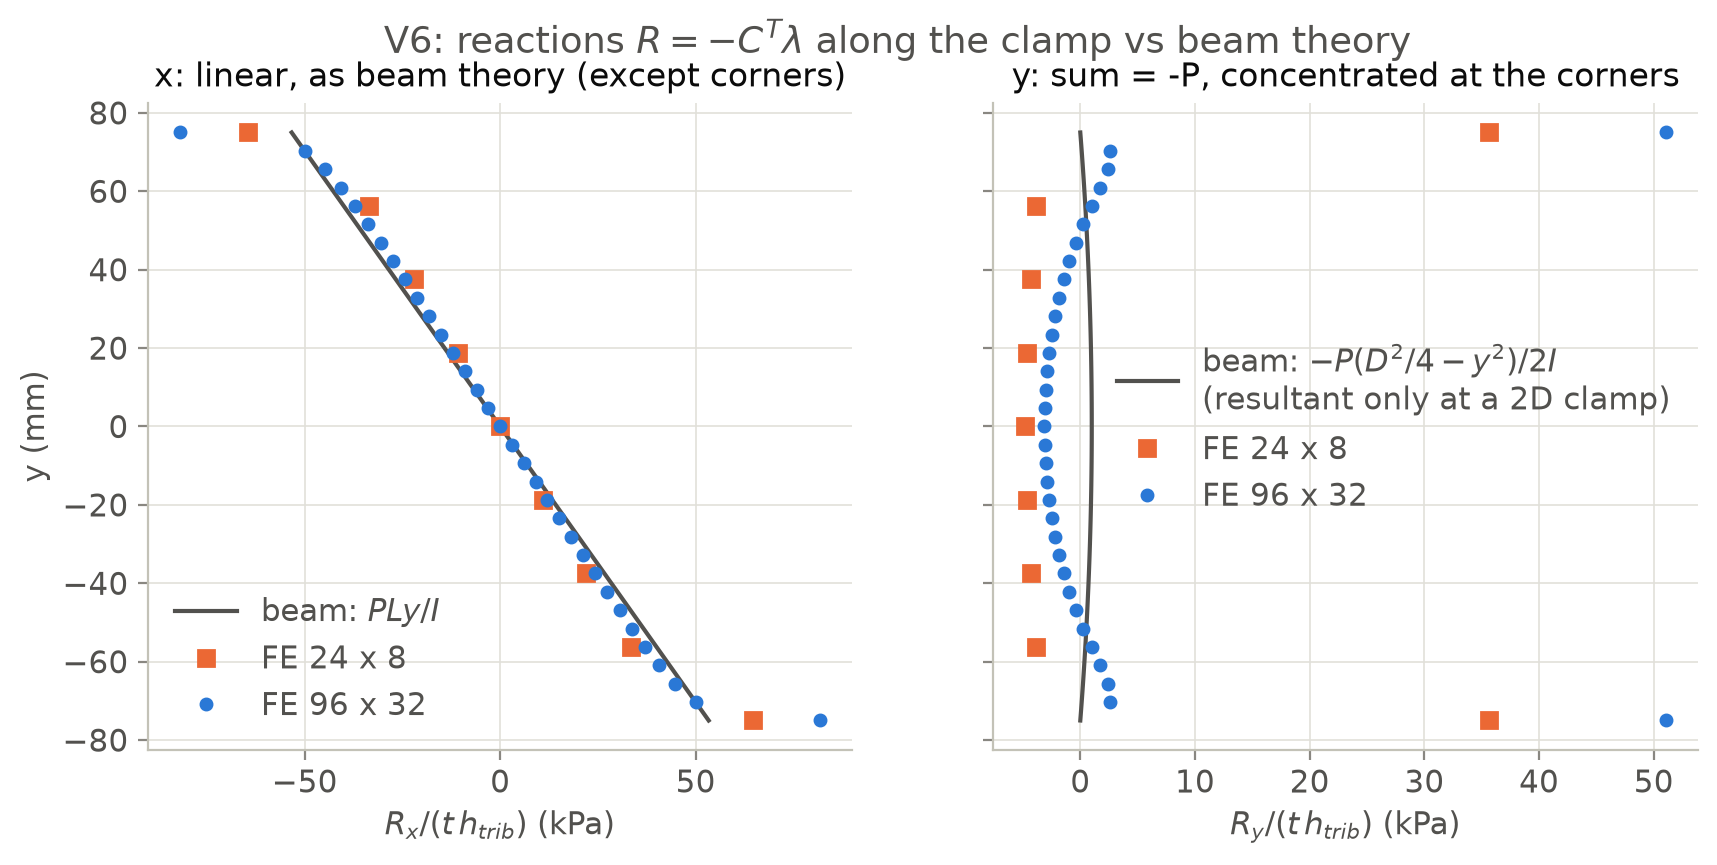
\includegraphics[width=0.72\linewidth]{reactions.png}\hfill
  \begin{minipage}[b]{0.26\linewidth}
    \footnotesize\raggedright
    $R_x$: linear, as beam theory ($PLy/I$); interior nodes within 5.4\% on $96\times32$.\\[5pt]
    Corner nodes: $t_x/(PLy/I)=$ 1.211, 1.536, 2.130 on $24\times8$, $96\times32$, $384\times128$; it keeps
    growing.\\[5pt]
    $R_y$: the sum is exactly $-P$, but it is concentrated at the corners. At a 2D clamp the parabola fixes
    only the resultant (Saint-Venant).\\[5pt]
    The clamped corners are \textbf{singular points} of 2D elasticity.
  \end{minipage}
  \vfill
  \src{figures/reactions.txt, figures/reactions.png.}
\end{frame}

% =====================================================================
\section{Conclusions}

\begin{frame}{Conclusions}
  \begin{itemize}
    \item \textbf{Lagrange multipliers behave exactly as the theory says}: the same displacements as elimination,
          and the multipliers \emph{are} the reactions, $\vR=-C^T\vlam$; statics holds to round-off on every mesh.
          Non-zero prescribed values ($\vg\ne\mathbf 0$) need no change to the code.
    \item \textbf{Scaling is essential}: unscaled, $\operatorname{cond}_2\approx10^{22}$ and about four digits are
          lost on an exact field; scaling by $\max\operatorname{diag}K$ makes the system as well conditioned as the
          eliminated one.
    \item \textbf{Q4 locks in bending}: one element gives 0.01445 of the Euler--Bernoulli deflection and $3\times1$
          gives 0.1155; in pure bending the error is exactly Cook Eq.~3.6-11.
    \item \textbf{Converged answer}: $-4.75532$ \textmu m $=0.99869\times$ Timoshenko $=1.00308\times$
          Euler--Bernoulli. Beam theory is not the exact 2D solution: the full clamp restrains warping and Poisson
          contraction at the root, and the load is a uniform traction. These effects scale like $(D/L)^2$, the
          same order as the shear term (0.44\%), so a 0.1--0.3\% gap is expected.
    \item \textbf{Every number has an analytical counterpart}, computed from its formula and checked by 109 tests;
          every closed form is derived symbolically.
  \end{itemize}
\end{frame}

\begin{frame}{Limitations}
  \begin{columns}[T]
    \begin{column}{0.48\textwidth}
      \textbf{Model}
      \begin{itemize}
        \item Linear elasticity, small displacements, plane stress
        \item One element type (Q4, full integration): fine meshes needed in bending
              (within 1\% of Timoshenko only from $96\times32$ on)
        \item Structured rectangular meshes, one load case
      \end{itemize}
    \end{column}
    \begin{column}{0.48\textwidth}
      \textbf{Interpretation}
      \begin{itemize}
        \item Stresses at the clamped corners are mesh-dependent (singularity, not resolved)
        \item The exact 2D solution for this clamp and load is outside the scope: beam theory is the
              reference, and the remaining gap is explained, not removed
        \item The order is observed for $h$ from $L/12$ to $L/384$; the corner singularity could lower it on much
              finer meshes
      \end{itemize}
    \end{column}
  \end{columns}
  \vspace{0.3em}
  \begin{block}{Reproduce everything}
    \small
    \begin{tabular}{@{}ll@{}}
      \texttt{python -m pytest -q} & the 109 tests \\
      \texttt{python run\_all.py} & every figure and table in figures/ \\
      \texttt{python -m checks.derivations} & the symbolic proofs \\
    \end{tabular}
  \end{block}
\end{frame}

\begin{frame}[plain]
  \centering
  \vspace{2.5em}
  {\Large\bfseries Thank you}\\[1em]
  {\large Questions?}\\[2.5em]
  \small\color{ink2}
  Backup slides: code map \textbullet\ symbolic proofs \textbullet\ the V5 hand solution \textbullet\
  why the unscaled condition number is $\sim10^{22}$
\end{frame}

% =====================================================================
\appendix

\begin{frame}{Backup: code map (equation $\to$ function $\to$ test)}
  \footnotesize
  \begin{tabular}{@{}L{0.34\textwidth}L{0.31\textwidth}L{0.29\textwidth}@{}}
    \toprule
    Equation / step & Code & Test \\
    \midrule
    Plane-stress $D$ & \texttt{fem/material.py} & \texttt{test\_q4.py} \\
    $N$, $[J]$, $B$, $k$ by Gauss & \texttt{fem/q4.py} & \texttt{test\_q4.py} (V2, V4) \\
    Mesh, DOF numbering & \texttt{fem/mesh.py}, \texttt{assemble.py} & all 2D tests \\
    $K=\sum L^Tk\,L$ (COO $\to$ CSR) & \texttt{fem/assemble.py} & \texttt{test\_cantilever.py} \\
    Consistent edge loads & \texttt{fem/loads.py} & \texttt{test\_cantilever.py}, \texttt{test\_exact\_field.py} \\
    $C$, scaled solve, $\vR=-C^T\vlam$ & \texttt{fem/lagrange.py} & \texttt{test\_bar1d.py}, \texttt{test\_cantilever.py} \\
    Cantilever driver & \texttt{fem/cantilever.py} & V5, V6 tests \\
    Stresses, $v(L,0)$, resultants, order, Richardson & \texttt{fem/post.py} & V3, V6 tests \\
    Closed forms V2--V5 & \texttt{checks/closed\_form.py} & \texttt{test\_q4.py}, \texttt{test\_one\_element.py} \\
    Beam theory & \texttt{checks/beam\_theory.py} & V4, V6 tests \\
    Symbolic proofs & \texttt{checks/derivations.py} & \texttt{test\_derivations.py} \\
    \bottomrule
  \end{tabular}
\end{frame}

\begin{frame}{Backup: what \texttt{checks/derivations.py} proves (sympy)}
  \begin{columns}[T]
    \begin{column}{0.49\textwidth}
      \begin{itemize}
        \item Plane-stress $D$ from 3D Hooke's law
        \item Exact $k$ of a rectangle; $2\times2$ Gauss reproduces it exactly; $k_{11}$, $k_{12}$
        \item Cook Eq.~3.6-11 from the two strain energies
        \item One-element cantilever: all displacements and all four reactions, minimising $\Pi$ over the four
              free DOFs (no symmetry assumed)
        \item Euler--Bernoulli by integrating $EIv''=M$; Timoshenko shear term; $I=tD^3/12$
        \item $\tau_{xy}$ from equilibrium, and $\int\tau_{xy}t\,dy=P$
      \end{itemize}
    \end{column}
    \begin{column}{0.49\textwidth}
      \begin{itemize}
        \item Bar: ODE, end conditions, support forces
        \item Uniform tension: $\bm\sigma=[\sigma_0,0,0]$ and the boundary conditions
        \item Consistent edge load $th\bar\tau/2$
        \item Lagrange $=$ elimination; $\vlam=-\vR$; $\vlam_s=\vlam/s$ under scaling
        \item Richardson's formula; $(\phi_1-\phi_2)/(\phi_2-\phi_3)=2^q$
      \end{itemize}
      \vspace{0.5em}
      \begin{block}{How it is used}
        Each derived expression is compared with the expression the code uses;
        \texttt{tests/test\_derivations.py} fails if any pair differs.
      \end{block}
    \end{column}
  \end{columns}
\end{frame}

\begin{frame}{Backup: the V5 hand solution in detail}
  Nodes 1 $(0,-b)$, 2 $(L,-b)$, 3 $(L,b)$, 4 $(0,b)$; $a=L/2$, $b=D/2$; nodes 1 and 4 clamped; $P/2$ on $v$ at 2 and 3.
  Symmetry: $u_3=-u_2=q$, $v_2=v_3=w$.
  \[
    u=q\,r\,\frac{1+s}{2},\quad v=w\,\frac{1+s}{2}\ \Rightarrow\
    \varepsilon_x=\frac{qr}{2a},\ \ \varepsilon_y=0,\ \ \gamma_{xy}=\frac{q(1+s)}{2b}+\frac{w}{2a}
  \]
  \[
    \Pi(q,w)=\frac{t\,ab}{2}\int_{-1}^{1}\!\!\int_{-1}^{1}\big(D_{11}\varepsilon_x^2+G\gamma_{xy}^2\big)\,ds\,dr-Pw
  \]
  \[
    \frac{\partial\Pi}{\partial q}=0,\ \frac{\partial\Pi}{\partial w}=0\ \Rightarrow\
    q=-\frac{3a^2P}{t(Ga^2+D_{11}b^2)},\qquad
    w=\frac{aP(D_{11}b^2+4Ga^2)}{tGb(Ga^2+D_{11}b^2)}
  \]
  With $D_{11}=E/(1-\nu^2)$, $G=E/(2(1+\nu))$, $a=L/2$, $b=D/2$ this is the $v_{tip}$ formula of V5, and
  $u_{top}=-u_{bottom}=-\dfrac{6PL^2(1-\nu^2)}{Et\,[L^2(1-\nu)+2D^2]}$.\\[4pt]
  Reactions: $\sum F_x=0$ and $\sum M_O=0$ give $R_{x1}+R_{x4}=0$ and $PL+b(R_{x1}-R_{x4})=0$, so $R_{x1}=-PL/D$;
  $\sum F_y=0$ and symmetry give $R_{y1}=R_{y4}=-P/2$.
\end{frame}

\begin{frame}{Backup: why the unscaled condition number is $\sim10^{22}$}
  With $C=[\,0\ \ I\,]$ (scaled by $s$), the exact inverse of the saddle-point matrix is, in the order $[\vd_f,\vd_c,\vlam_s]$:
  \[
    A_s^{-1}=\begin{bmatrix}
      K_{ff}^{-1} & 0 & -K_{ff}^{-1}K_{fc}/s\\
      0 & 0 & I/s\\
      -K_{cf}K_{ff}^{-1}/s & I/s & \big(K_{cf}K_{ff}^{-1}K_{fc}-K_{cc}\big)/s^2
    \end{bmatrix}
  \]
  \begin{itemize}
    \item The last block is minus the stiffness the supports see: as large as $K$ ($\sim10^{11}$ N/m)
    \item $s=1$: $\|A\|\sim\|K\|\sim10^{11}$ and $\|A^{-1}\|\gtrsim10^{11}$, so $\operatorname{cond}\sim10^{22}$
    \item $s=\max\operatorname{diag}K$: that block shrinks to $\sim1/s$ and the coupling blocks are divided by $s$;
          $\|A_s^{-1}\|\approx\|K_{ff}^{-1}\|$, so $\operatorname{cond}(A_s)\approx\operatorname{cond}(K_{ff})$
          (measured within 3\%)
  \end{itemize}
  \src{Checked numerically with this exact inverse and with a 50-digit SVD (mpmath) on $3\times1$ and $6\times2$.}
\end{frame}

\end{document}
